We now give an overview of common data structures used in \BoxLib, followed by a simple
example written in both Fortran90 and C++ that makes use of these structures.
The example advances two scalar variables in time on a single level with multiple 
grids (no AMR) and produces plotfiles.

\section{Overview of Data Structures}

\BoxLib\ contains the most fundamental objects used to construct parallel
block-structured AMR applications.
At each level of refinement, the region covered by that level is divided
into grids, or boxes.  The entire computational domain is covered by
the coarsest (base) level of refinement (called level $\ell=0$ in C++ 
and called level $\ell=1$ in Fortran90) and can be represented on one
grid or divided into many grids.
Higher levels of refinement have cells that are finer by a ``refinement ratio''
of either 2 or 4 (in C++) or 2 (in Fortran90).  The grids are properly nested in the sense that the union 
of grids at level $\ell+1$ is contained in the union of grids at level $\ell$.
Furthermore, the containment is strict in the sense that, except at physical 
boundaries (i.e., domain boundaries that are not periodic),
the level $\ell$ grids are large enough to guarantee that there is
a border at least $n_{\rm buffer}$ (typically 4) level $\ell$ cells wide surrounding each level
$\ell +1$ grid (grids at all levels are allowed to extend to the physical
boundaries so the proper nesting is not strict there).  See Figure \ref{fig:AMR}
for a sample two-dimensional grid structure.\\
%%%%%%%%%%%%%%%%%%%%%%%%%%%%%%%%%%%%%
\begin{figure}[htb]
\centering
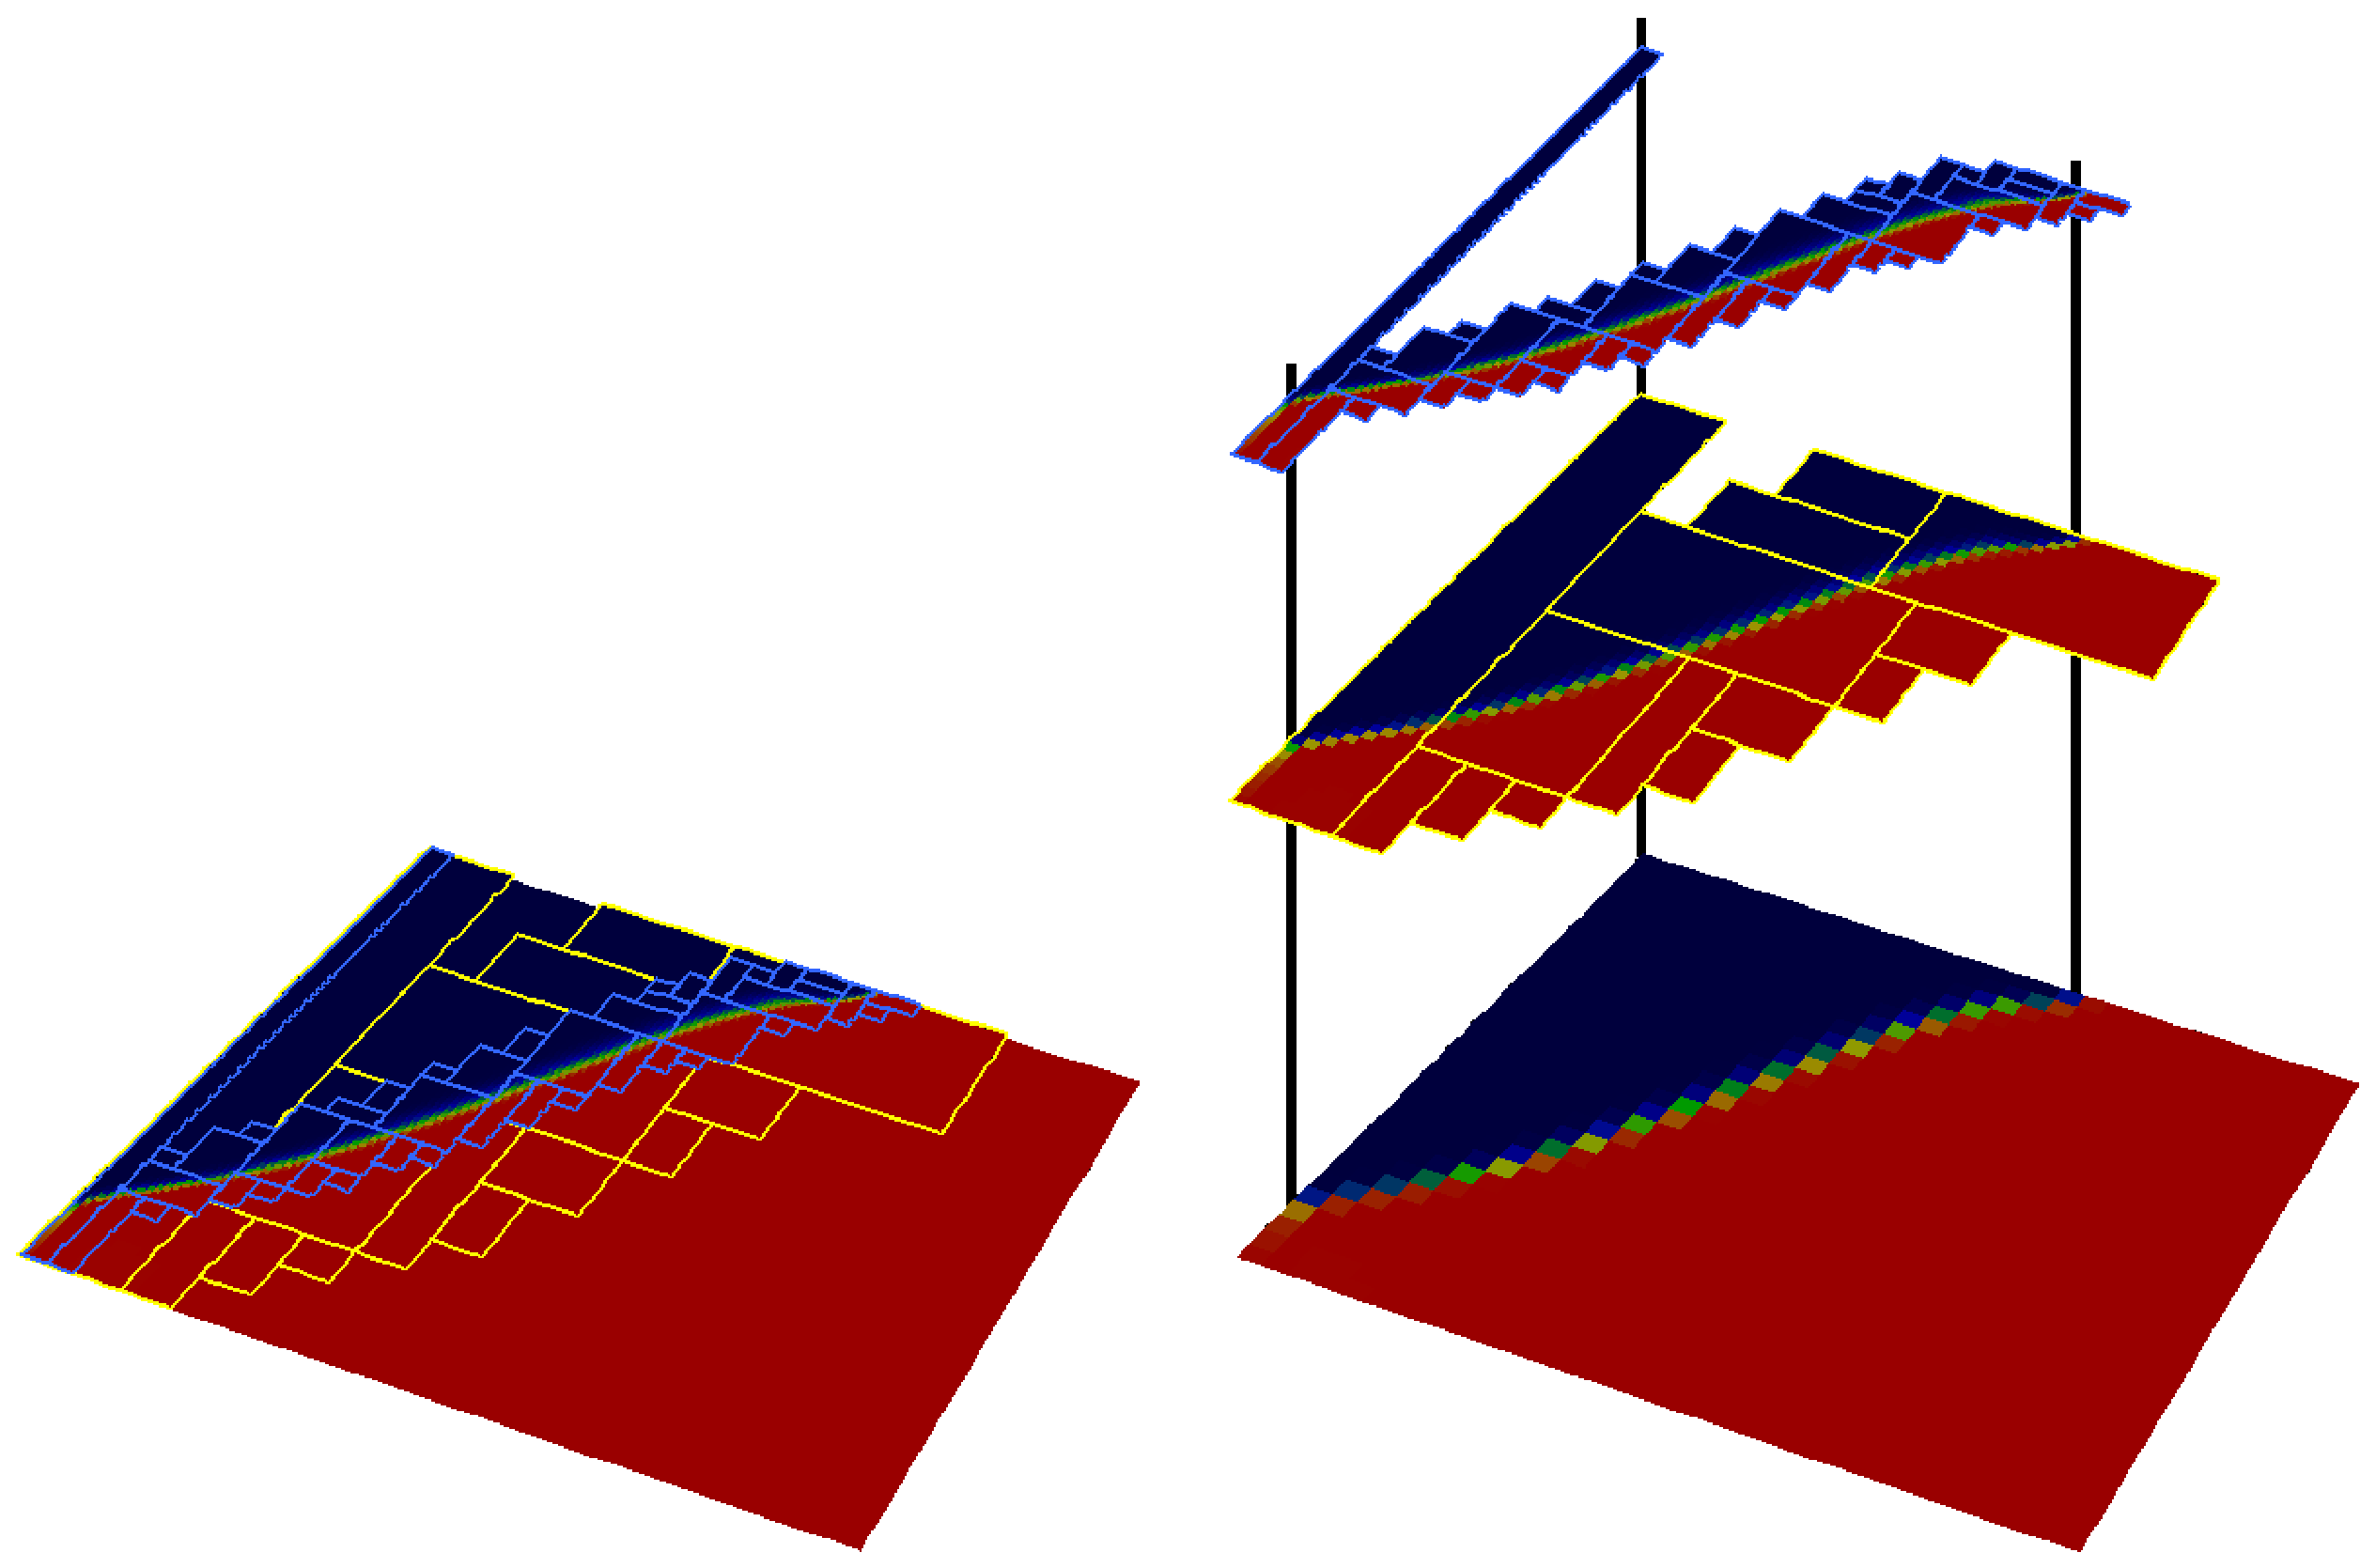
\includegraphics[width=4in]{./Introduction/AMR}
\caption{\label{fig:AMR}Sample grid structure with two levels of refinement.  These
grids satisfy the requirements that the base grid (i.e., the coarsest level)
covers the entire computational domain 
and the grids are properly nested.  Note that refined grids are allowed to extend to physical
(non-periodic) domain boundaries without coarser buffer cells.}
\end{figure}
%%%%%%%%%%%%%%%%%%%%%%%%%%%%%%%%%%%%%

On a grid, the data can be stored at cell-centers, faces, edges (in three dimensions), or
corners.  In \BoxLib, data that is on an face is termed `nodal'
in that one direction (see Figure~\ref{fig:dataloc}).  In three-dimensions (not pictured),
data that is nodal in two directions is said to live on edges.  Data that is nodal in
all directions lives on the corners of cells (commonly referred to as the nodes).
\BoxLib\ uses $0$-based spatial indexing, and for data that is nodal in one or more direction,
the integer index corresponds to the lower boundary in that direction (see Figure~\ref{fig:dataloc}).
In our \BoxLib\ applications, the state data (velocity, density, 
species, $\ldots$) is typically cell-centered.  Fluxes are typically nodal in exactly
one direction (i.e.~they are face-centered).  A few quantities are nodal in all 
directions (e.g.~the pressure in the low Mach number projection methods).
%%%%%%%%%%%%%%%%%%%%%%%%%%%%%%%%%%%%%
\begin{figure}[htb]
\centering
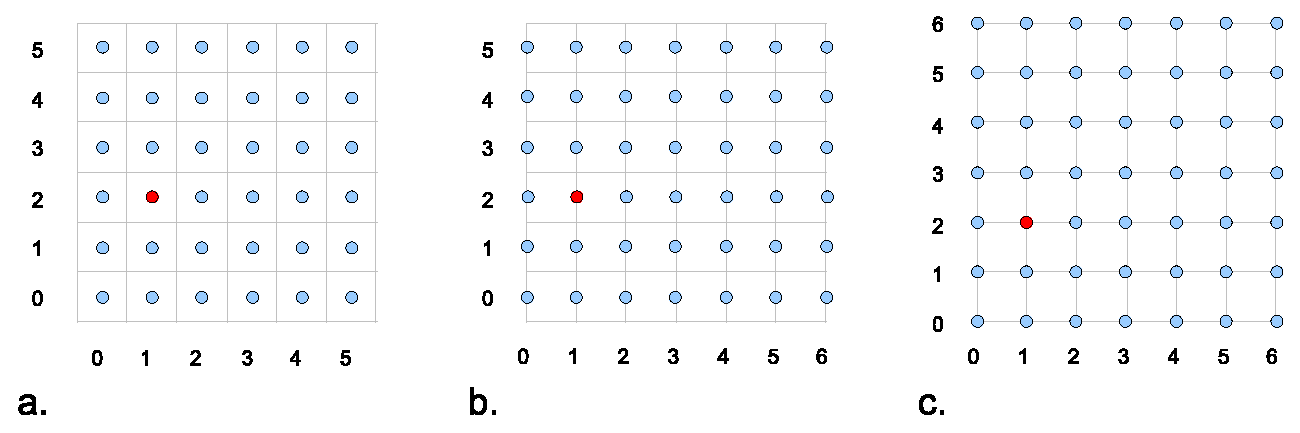
\includegraphics[width=6.5in]{./Introduction/data_loc2}
\caption{\label{fig:dataloc} Some of the different data-centerings in two dimensions:
(a) cell-centered, (b) face-centered, i.e., nodal in one dimensions ($x$) only, and (c) corner/nodal,
i.e., nodal in all dimensions.  Note that for data that is nodal in one or more direction,
the integer index corresponds to the lower boundary in that direction.
Also note that \BoxLib\ uses $0$-based indexing, e.g., in each of these centerings, 
the red point has the same indices:\ (1,2).
Not shown is the case where data is nodal in the $y$-direction only.  
Also not shown is the three-dimensional edge-centered case, where the data
is nodal in exactly two directions.}
\end{figure}
%%%%%%%%%%%%%%%%%%%%%%%%%%%%%%%%%%%%%

\begin{itemize}
\item In C++ \BoxLib, we must specify the number of spatial dimensions (1, 2, or 3), 
{\tt DIM}, at compile-time.  The code that will be built is specifically designed to 
run only with that number of dimensions.
\item In Fortran90 \BoxLib, we build dimension-independent code at compile-time, 
and tell the program the dimensionality of the problem via a runtime inputs file.
\end{itemize}

To simplify the description of the underlying AMR grid, \BoxLib\
provides a number of classes.  We now briefly summarize some of the major
classes.

\subsection{\IntVect}

\IntVect s are {\tt DIM}-tuples of integers that are used to define
indices in space.  In C++, an example of an \IntVect\ in 2D would be
(C++ source code will be shaded blue):
\begin{lstlisting}[backgroundcolor=\color{light-blue}]
IntVect iv(3,5);
\end{lstlisting}
In Fortran90, we don't use \IntVect s, but instead use standard
arrays of integers (Fortran90 source code will be shaded green):
\begin{lstlisting}[backgroundcolor=\color{light-green}]
integer :: iv(2)
iv(1) = 3
iv(2) = 5
\end{lstlisting}

\subsection{\BoxType}

A \BoxType\ is simply a rectangular domain in space and does not hold any data.
A \BoxType\ contains the indices of its low end and high end, 
{\tt IntVect lo} and {\tt IntVect hi}.
\begin{itemize}
\item In C++, a \BoxType\ also
contains an {\tt IndexType} (cell-centered, face-centered, or nodal) for each
spatial direction.
\item In Fortran90, a \BoxType\ also contains the dimensionality 
of the \BoxType.
\end{itemize}
To build a \BoxType\ in C++ use:
\begin{lstlisting}[backgroundcolor=\color{light-blue}]
// define a box with bounds (0,0) to (15,15) in 2D
IntVect lo(0,0), hi(15,15);
Box bx(lo,hi);
\end{lstlisting}
To build a \BoxType\ in Fortran90 use:
\begin{lstlisting}[backgroundcolor=\color{light-green}]
type(box) :: bx
integer   :: iv_lo(2), iv_hi(2)
iv_lo(1:2) = (/ 0, 0 /)
iv_hi(1:2) = (/ 15, 15 /)
bx = make_box(lo,hi)
\end{lstlisting}

The computational domain is divided into non-overlapping grids.  
The collection of grids at the same resolution comprise a level.
Figure~\ref{fig:boxes} shows three grids at the same level of
refinement.  Note that this figure cannot represent the base level of refinement,
since it would require that the grids span the problem domain.
The position of the grids is with respect to a global
index space that covers the entire domain at that level and uses 0-based indexing.
For example, the \BoxType\ associated with grid 1 
in the figure has {\tt lo} = (2,6) and {\tt hi} = (5,13).
%%%%%%%%%%%%%%%%%%%%%%%%%%%%%%%%%%%%%
\begin{figure}[tb]
\centering
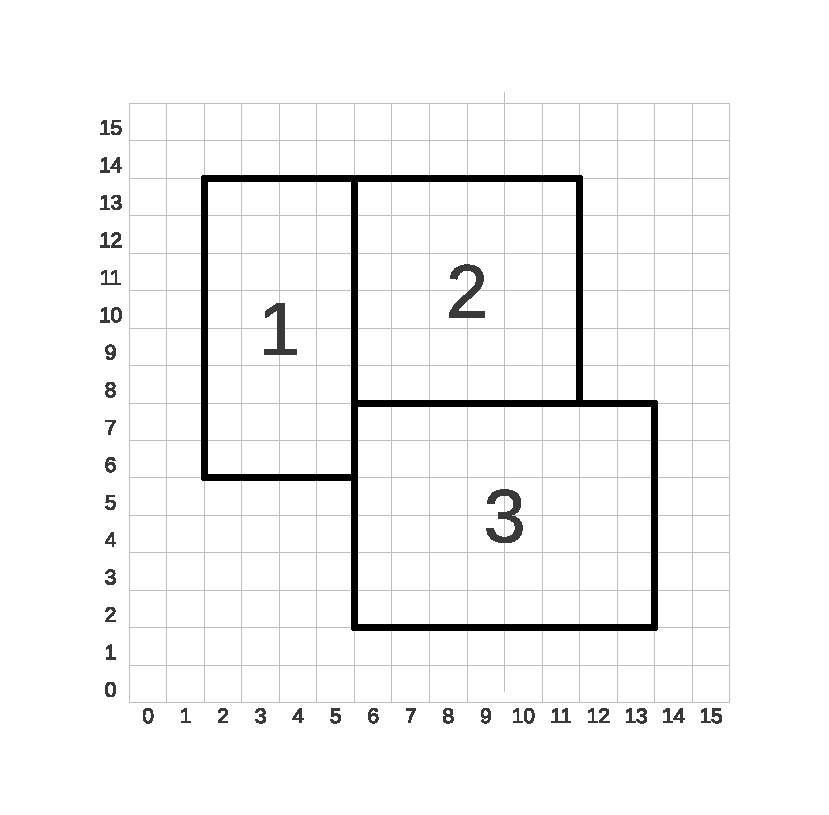
\includegraphics[width=4.0in]{./Introduction/index_grid2}
\caption{\label{fig:boxes} Three boxes that comprise a single level.
At this level of refinement, the domain is 16$\times$16 cells and
the global index space runs from 0 to 15 in each coordinate direction.
Note that these grids cannot be at the coarsest level,
since it would require that the grids span the problem domain.}
\end{figure}
%%%%%%%%%%%%%%%%%%%%%%%%%%%%%%%%%%%%%

\begin{itemize}
\item Example: For a simulation with 32 cells in each direction at the coarsest level,
the global index space for the coarsest level runs from 0 to 31 in each coordinate
direction.  Assuming refinement ratios of 2, the next finer level 
will have a global index space running from 
0 to 63 in each coordinate direction (corresponding to $64 \times
64$ zones if fully refined), and the next finer level will have a global index
space running from 0 to 127 in each coordinate direction
(corresponding to $128\times 128$ zones if fully refined).
\end{itemize}

\subsection{\BoxArray}

A \BoxArray\ is an array of \BoxType es.  The size of the array is the 
number of \BoxType es in the \BoxArray.  Suppose your problem domain
has lo indices (0,0) and hi indices (15,15), and you want to define
a \BoxArray\ to contain four $8\times 8$ boxes to cover the problem domain.
In Fortran90, you could do the following:
\begin{lstlisting}[backgroundcolor=\color{light-green}]
integer        :: lo(2), hi(2)
type(box)      :: bx(4)
type(boxarray) :: ba
lo(1:2) = (/ 0, 0 /)
hi(1:2) = (/ 7, 7 /)
bx(1) = make_box(lo,hi)
lo(1:2) = (/ 8, 0 /)
hi(1:2) = (/ 15, 7 /)
bx(2) = make_box(lo,hi)
lo(1:2) = (/ 0, 8 /)
hi(1:2) = (/ 7, 15 /)
bx(3) = make_box(lo,hi)
lo(1:2) = (/ 8, 8 /)
hi(1:2) = (/ 15, 15 /)
bx(4) = make_box(lo,hi)
call boxarray_build_v(ba,bx)
\end{lstlisting}
This is rather cumbersome, so instead we use built-in \BoxLib\ functions to
divide a single box into smaller boxes to build the same \BoxArray:
\begin{lstlisting}[backgroundcolor=\color{light-green}]
type(boxarray) :: ba
integer        :: lo(2), hi(2)
type(box)      :: bx
lo(1:2) = 0
hi(1:2) = 15
bx = make_box(lo,hi)
call boxarray_build_bx(ba,bx)  ! ba has one 16^2 box
call boxarray_maxsize(ba,8)    ! ba now has four 8^2 boxes
\end{lstlisting}
The define the same \BoxArray in C++, first define {\tt bx} as before, then
\begin{lstlisting}[backgroundcolor=\color{light-blue}]
// define a box with bounds (0,0) to (15,15) in 2D
BoxArray ba(bx);  // ba has one 16^2 box
ba.maxSize(8);    // ba now has four 8^2 boxes
\end{lstlisting}

\subsection{\layout\ (Fortran90 Only)}

A \layout\ is a more intelligent \BoxArray,
since it contains a \BoxArray\ as well
as the associated processor assignments, \BoxType\ connectivity, whether or not the 
domain is periodic in each direction, and many other
parallel constructs.  In the simplest case, if we have a \BoxArray\ {\tt ba} (obtained
from the example above), a \layout\ can be defined using:
\begin{lstlisting}[backgroundcolor=\color{light-green}]
type(layout)   :: la
type(box)      :: pd
type(boxarray) :: ba
logical        :: is_periodic(2)

is_periodic(1:2) = .true.
call layout_build_ba(la,ba,pd,is_periodic)
\end{lstlisting}
Here, {\tt pd} is a box that spans the entire domain.

In C++, the information that is contained in the Fortran90 \layout\ is part of
the \MultiFab\ class.

\subsection{\Geometry\ (C++ Only)}

\Geometry\ is a class that stores the physical coordinates and the indices of the
lo and hi corners of the problem domain, the coordinate system of the problem
(Cartesian, RZ, or spherical) as well as the periodicity.  To define a \Geometry\
object, first build the \BoxArray\ {\tt ba} above, then
\begin{lstlisting}[backgroundcolor=\color{light-blue}]
// This stores the physical coordinates of the problem domain
RealBox real_box;
for (int n = 0; n < BL_SPACEDIM; n++)
{
  real_box.setLo(n,-1.0);
  real_box.setHi(n, 1.0);
}

// This says we are using Cartesian coordinates
int coord = 0;

// This says the domain is periodic in each direction
int is_per[BL_SPACEDIM];
for (int i = 0; i < BL_SPACEDIM; i++)
{
  is_per[i] = 1;
}

// Define a Geometry object to store problem domain physical coordinates,
// incides, coordinate system, and periodicity
Geometry geom;
geom.define(bx, &real_box, coord, is_per);
\end{lstlisting}

\subsection{\FArrayBox}

A \FArrayBox\ (or \Fab) is a ``Fortran array box'' that holds data.  It contains the
\BoxType\ that it is built on as well as a pointer to the data 
that can be sent to a Fortran routine.
In Fortran90, \Fab\ data is stored in a four-dimensional array,
{\tt (nx,ny,nz,nc)} in size, regardless of the dimensionality of the
problem.  Here {\tt nc} is the number of components, for instance
representing different fluid variables.  For 2D problems, {\tt nz=1}.
In C++, \Fab\ data is stored in a one-dimensional array, and we pass
shape information into Fortran90 subroutines when we need to access
the data.

In \BoxLib, we don't usually deal with 
\Fab s alone, but rather through \MultiFab s, described next.

\subsection{Floating point data}

Floating point data in C++ is declared as {\tt Real} which is {\tt
typedef} to either {\tt float} or {\tt double} depending on how {\tt
PRECISION} is set in the {\tt GNUmakefile}.  This is defined in {\tt
REAL.H}.  In Fortran90, the {\tt bl\_types} module defines a type {\tt dp\_t} that
is double precision.  Floating point types should be declared using
{\tt real (kind=dp\_t)}.


\section{The \MultiFab}
\MultiFab s are so important that we will give them their own section.
A \MultiFab\ is a collection of all the \Fab s at the same level of
refinement.
\begin{itemize}
\item In C++, a \MultiFab\ is defined using a \BoxArray,
number of components, and number of ghost cells that each \Fab\
will have.
\item In Fortran90, a \MultiFab\ is defined using a \layout,
number of components, and number of ghost cells that each \Fab\
will have.
\end{itemize}
A \MultiFab\ has a ``valid'' region that is defined by 
the \BoxArray~or \layout.  Each \Fab\ in the \MultiFab\ is built large enough 
to hold valid data and ghost cell data, and thus the \BoxType\ associated with
each \Fab\ is a grown version of the corresponding \BoxType\ from the \BoxArray.
Thus, a \Fab\ has no concept 
of ghost cells, it merely has a single \BoxType\ that identifies it.\\

To build a \MultiFab, we require a \layout\ (in Fortran90) or a \BoxArray\ (in C++).
In Fortran90, using the \layout\ built above, we build a \MultiFab\ using:
\begin{lstlisting}[backgroundcolor=\color{light-green}]
type(multifab) :: data
call multifab_build(data,la,2,6) ! build a multifab with 2 components 
                                 ! and 6 ghost cells

...                              ! do fun stuff with the data

call multifab_destroy(data)      ! free up memory to prevent leaks
\end{lstlisting}
In C++, using the \BoxArray\ built above, you could either directly 
build a \MultiFab\ using:
\begin{lstlisting}[backgroundcolor=\color{light-blue}]
MultiFab data(ba,2,6);                     // build a MultiFab
\end{lstlisting}
or a pointer to a \MultiFab\ using:
\begin{lstlisting}[backgroundcolor=\color{light-blue}]
MultiFab* data = new MultiFab(ba,2,6);     // build pointer to MultiFab

...                                        // do fun stuff with the data

delete data;                               // need to free the memory
\end{lstlisting}
In the C++ tutorial {\tt BoxLib/Tutorials/HeatEquation\_EX1\_C/}, we use
the {\tt PArray} class, which manages memory under the covers
to prevent memory leaks:
\begin{lstlisting}[backgroundcolor=\color{light-blue}]
// define a multifab with 2 components and 6 ghost cells
// We use the PArray class to help manage the memory
// (auto deallocation to prevent memory leaks)

// the "1" means only 1 MultiFab; you can declare more if needed
PArray <MultiFab> data(1,PArrayManage);

// build the "0th" MultiFab in the PArray
data.set(0, new MultiFab(ba, 2, 6));
\end{lstlisting}
In the next section we will demonstrate how to access \MultiFab\ data.

\section{First Example - Accessing \MultiFab\ Data}

Here is a complete Fortran90 program that shows you how to build a 
\MultiFab\ and access its data.  The complete source code, which you can build and run,
is in {\tt BoxLib/Tutorials/GettingStarted\_F/}.  It consists of two source code files; {\tt main.f90}:
\lstinputlisting[backgroundcolor=\color{light-green}]{../../Tutorials/GettingStarted_F/main.f90}
and {\tt work\_on\_data.f90}:
\lstinputlisting[backgroundcolor=\color{light-green}]{../../Tutorials/GettingStarted_F/work_on_data.f90}

Here is a complete C++ program that shows you how to build a 
\MultiFab\ and access its data.  The complete source code, which you can build and run,
is in {\tt BoxLib/Tutorials/GettingStarted\_C/}.  It consists of two source code files; {\tt main.cpp}:
\lstinputlisting[backgroundcolor=\color{light-blue}]{../../Tutorials/GettingStarted_C/main.cpp}
and {\tt work\_on\_data\_2d.f90}:
\lstinputlisting[backgroundcolor=\color{light-blue}]{../../Tutorials/GettingStarted_C/work_on_data_2d.f90}

Note that in C++, {\tt work\_on\_data} calls a Fortran90 subroutine which is nearly
identical to the Fortran90 example given above.  The only difference is the subroutine
name cannot have the \_2d or \_3d in its name.  Thus, the 2d and 3d versions
are both named {\tt subroutine work\_on\_data}, and must be written in
different .f90 files, where the make system determines which version to compile
based on {\tt DIM}.\\

The {\tt multifab\_fill\_boundary} and {\tt FillBoundary} functions 
fill all ghost cells on periodic domain boundaries, as well as interior
ghost cells with values that can simply be copied from the valid region of a neighboring
grid at the same level of refinement.  For single-level problems that are periodic
in all directions, these functions fill all ghost cells.  We will discuss
non-periodic domain boundaries and fine grid ghost cells near coarse-fine interfaces
in Chapter \ref{Sec:Boundary Conditions} for Fortran90.

\subsection{Other \MultiFab\ Functions}
\begin{itemize}
\item {\tt setVal} sets the \MultiFab\ data to a particular value.
\end{itemize}
In Fortran90, use:
\begin{lstlisting}[backgroundcolor=\color{light-green}]
! set all variables to 0.0; ``all=.true.'' means set the ghost cells also
call setval(data,0.d0,all=.true.)
\end{lstlisting}
In C++, use:
\begin{lstlisting}[backgroundcolor=\color{light-blue}]
data.setVal(0.0);  // set all variables to 0.0, including ghost cells
\end{lstlisting}
\begin{itemize}
\item {\tt copy} copies data from one \MultiFab\ to another.
\end{itemize}
In Fortran90, use:
\begin{lstlisting}[backgroundcolor=\color{light-green}]
! copy components 1 and 2 from data_src into data_dest, 
! including the ghost cells. calling sequence is 
! (1) destination multifab, (2) first component of destination, 
! (3) source multifab, ! (4) first component of source, 
! (5) number of components, (6) ghost cells
call multifab_copy_c(data_dest,1,data_src,1,2,6)
\end{lstlisting}
In C++, use:
\begin{lstlisting}[backgroundcolor=\color{light-blue}]
// copy components 0 and 1 from data_src into data_dest, 
// including the ghost cells. calling sequence is 
// (1) destination multifab, (2) source multifab, 
// (3) first component of destination, (4) first component of source, 
// (5) number of components, (6) ghost cells
MultiFab::Copy(data_dest,data_src,0,0,2,6)
\end{lstlisting}
There are many other subroutines available for adding, subtracting, multiplying, etc.,
components of \MultiFab s, finding the min/max value, norms, number of cells, etc.
Refer to {\tt BoxLib/Src/F\_BaseLib/multifab\_f.f90} or 
{\tt BoxLib/Src/C\_BaseLib/MultiFab.H} for a complete listing.

\section{Second Example - Explicit Heat Equation}
We now provide a complete tutorial code that uses some concepts discussed above.
The code also writes plotfiles that can be viewed, and can be run in parallel if you
are working on a machine with MPI and/or OpenMP support.
\begin{itemize}
\item The Fortran90 version of this example is contained in {\tt BoxLib/Tutorials/HeatEquation\_EX1\_F/}.
\item The C++ version of this example is contained in {\tt BoxLib/Tutorials/HeatEquation\_EX1\_C/}.
\end{itemize}

In this example, we advance the equation:
\begin{equation}
\frac{\partial\phi}{\partial t} = \nabla^2 \phi; \quad \phi(t=0) = 1 + e^{-100r^2},
\end{equation}
on a domain from [-1,1] in each spatial direction, where $r$ is the distance
to the point $(x,y,z) = (0.25,0.25,0.25)$.  Note that we are placing the
initial Gaussian profile slightly off-center.  This asymmetry will be important
in later sections when we examine the effects of non-periodic boundary conditions.
We will assume that $\Delta x = \Delta y = \Delta z$ and use a fixed
time step with $\Delta t = 0.9\Delta x^2$.  We begin with a simple 
single-level, forward Euler discretization, periodic boundary conditions,
and no refinement (i.e., only one level).\\

The basic time-advancement strategy uses the following temporal discretization:
\begin{equation}
\frac{\phi_{ij}^{n+1} - \phi_{ij}^n}{\Delta t} = \left[\nabla\cdot(\nabla\phi)\right]_{ij}.
\end{equation}
In the explicit case, we first compute $\nabla\phi$, at faces using:
\begin{equation}
(\nabla\phi)_{i+\myhalf,j} = \frac{\phi_{i+1,j}^n-\phi_{ij}^n}{\Delta x}.
\end{equation}
We will refer to these face-centered gradients as ``fluxes''.
Next, we compute the update by taking the divergence of these fluxes,
\begin{equation}
\left[\nabla\cdot(\nabla\phi)\right]_{ij} = \frac{(\nabla\phi)_{i+\myhalf,j}-(\nabla\phi)_{i-\myhalf,j}}{\Delta x} + \frac{(\nabla\phi)_{i,j+\myhalf}-(\nabla\phi)_{i,j-\myhalf}}{\Delta y}.
\end{equation}
Note that the overall update could be expressed as a 5-point (in 2D) or 7-point (in 3D) 
Laplacian stencil,
but here use a flux divergence formulation because it will enable a more natural 
extension to multiple levels of refinement, where we will be concerned with
conservation across levels.  Note that in this explicit case, since $\Delta x = \Delta y$, 
the Laplacian reduces to the standard five point stencil in two dimensions
(seven point stencil in three dimensions).\\

\subsection{Fortran90}

Since the fluxes live on faces, we need face-centered \MultiFab s, i.e.,
\MultiFab s that are nodal in one spatial direction.  In {\tt advance.f90},
we build them as follows:
\begin{lstlisting}[backgroundcolor=\color{light-green}]
! an array of multifabs; one for each direction
type(multifab) :: flux(phi%dim) 

! build the flux(:) multifabs
do i=1,dm
   ! flux(i) has 1 component, 0 ghost cells, and is nodal in direction i
   call multifab_build_edge(flux(i),phi%la,1,0,i)
end do
\end{lstlisting}

In the problem directory, you will see the following files:
\begin{itemize}
\item {\tt GNUmakefile}

This contains compiler settings and directories required by the make system to build the code.

  \begin{itemize}

    \item {\tt BOXLIB\_HOME}

    Change this to point to the \BoxLib\ home directory.  Alternatively, you can define {\tt BOXLIB\_HOME}
    as an environment variable on your system and this line will be ignored.

    \item {\tt NDEBUG} ('{\tt t}' or '{\tt <blank>}') for TRUE or FALSE
      
    ``not debug'' (we know, confusing).  If '{\tt t}', modifies compiler flags to build a 
    more optimized version of the code.  The program will run faster, but have fewer 
    runtime error checks.

    \item {\tt MPI} ('{\tt t}' or '{\tt <blank>}')

    Indicate whether you want your executable to be MPI-compatible.  MPI must be installed on your
    machine in order to use this, and you must modify some of the make scripts, as will be 
    discussed later.

    \item {\tt OMP} ('{\tt t}' or '{\tt <blank>}')

    Turns on OpenMP compiler flags to compile in any OpenMP directives in the code.
    We will discuss OpenMP further in Section \ref{Sec:OpenMP}.

    \item {\tt PROF} ('{\tt t}' or '{\tt <blank>}')

    Turns on timer compilation flags.  Timers are useful for optimizing your code since they tell you 
    what subroutines are taking the most time and require more optimization.  Note that you still have 
    to write timers into your code.  Documentation for timers is coming soon!

    \item {\tt COMP} ('{\tt gfortran}, {\tt Intel}, $\ldots$)'

    The Fortran compiler.  Supported options include {\tt gfortran}, {\tt Intel}, 
    and {\tt Cray}.

    \item {\tt MKVERBOSE} ('{\tt t}' or '{\tt <blank>}')

    Verbosity of compile-time output.

  \end{itemize}

\item {\tt GPackage.mak}

List of local files needed to be included in the build.  The {\tt GNUmakefile} points to this.

\item {\tt main.f90}, {\tt init\_phi.f90}, {\tt advance.f90}, {\tt write\_plotfile.f90}

Source code that is not within the {\tt BoxLib/Src/} tree.  Note that 
if a file that exists in the
{\tt BoxLib/Src/} tree also exists in the local directory, the local copy takes precedence
as long as the {\tt GNUmakefile} lists your local directory as a {\tt VPATH\_LOCATIONS} 
before the \BoxLib\ source code directory, {\tt BoxLib/Src/F\_BaseLib}.

\item {\tt inputs\_2d}, {\tt inputs\_3d}

Input files to customize the simulation parameters.

\end{itemize}

To build the code, edit the {\tt GNUmakefile} and simply type ``{\tt make}''.  An 
executable will appear that has some indication (but not complete)
about what setting you used in the {\tt GNUmakefile}.  To run the code on a single processor,
simply type, for example (terminal commands and non-source code files are shaded in red),
\begin{lstlisting}[backgroundcolor=\color{light-red}]
./main.Linux.gfortran.exe inputs_2d
\end{lstlisting}
The program will complete and there will be a series of plotfiles, e.g., {\tt plt00000}, 
{\tt plt00100}, etc., in the run directory.  You can visualize the data 
and make animations using {\tt VisIt} (available at {\tt https://wci.llnl.gov/codes/visit/});
refer to Section \ref{Sec:VisIt}.

\subsection{C++}
The C++ version of this example is contained in {\tt BoxLib/Tutorials/HeatEquation\_EX1\_C/}.

\begin{itemize}
\item {\tt GNUmakefile}

This contains compiler settings and directories required by the make system to build the code.

  \begin{itemize}

    \item {\tt BOXLIB\_HOME}

    Change this to point to the \BoxLib\ home directory.  Alternatively, you can define {\tt BOXLIB\_HOME}
    as an environment variable on your system and this line will be ignored.

    \item {\tt DEBUG} ('{\tt TRUE}' or '{\tt FALSE}')
      
    Debug mode.  If 'FALSE', modifies compiler flags to build a more optimized version of the code.
    The program will run faster, but have fewer runtime error checks.

    \item {\tt USE\_MPI} ('{\tt TRUE}' or '{\tt FALSE}')

    Indicate whether you want your executable to be MPI-compatible.  MPI must be installed on your
    machine in order to use this, and you must modify some of the make scripts, as will be 
    discussed later.

    \item {\tt USE\_OMP} ('{\tt TRUE}' or '{\tt FALSE}')
    
    Turns on OpenMP compiler flags to compile in any OpenMP directives in the code.
    We will discuss OpenMP further in Chapter \ref{Sec:OpenMP}.

    \item {\tt PROFILE} ('{\tt TRUE}' or '{\tt FALSE}')

    Turns on timer compilation flags.  Timers are useful for optimizing your code since they tell you 
    what subroutines are taking the most time and require more optimization.  Note that you still have 
    to write timers into your code.  Documentation for timers is coming soon!

    \item {\tt COMP} ('{\tt g++}, {\tt Intel}, $\ldots$)'

    The C++ compiler.  Supported options include {\tt g++}, {\tt Intel}, and
    {\tt Cray}.

    \item {\tt FCOMP} ('{\tt gfortran}, {\tt Intel}, $\ldots$)'

    The Fortran compiler.  Supported options include {\tt g++}, {\tt Intel}, and
    {\tt Cray}.

    \item {\tt DIM} ('1', '2', or '3')

    Dimensionality of the problem.  Unlike Fortran90, you need to set this in the C++ version.

    \item {\tt PRECISION} ('{\tt DOUBLE}' or '{\tt FLOAT}')

    Precision of real numbers.  You can use {\tt FLOAT} for single-precision real numbers to save memory.

    \item {\tt EBASE} ('{\tt main}', $\ldots$)

    The executable string will begin with this.

  \end{itemize}

\item {\tt Make.package}

List of local files needed to be included in the build.  The {\tt GNUmakefile} points to this.

\item {\tt main.f90}, {\tt writePlotFile.cpp}, {\tt writePlotFile.H}, {\tt init\_phi\_2d.f90},
      {\tt init\_phi\_3d.f90}, {\tt advance\_2d.f90}, {\tt advance\_3d.f90}

Source code that is not within the {\tt BoxLib/Src/} tree.  Note that if a file that 
exists in the
{\tt BoxLib/Src/} tree also exists in the local directory, the local copy takes precedence
as long as the {\tt GNUmakefile} lists your local directory in the {\tt include} line before
before the \BoxLib\ source code directories.

\item {\tt inputs\_2d}, {\tt inputs\_3d}

Input files to customize the simulation parameters.

\end{itemize}

To build the code, simply type ``{\tt make}''.  An exectubale will appear that has some indication (but not complete)
about what setting you used in the {\tt GNUmakefile}.  To run the code on one processor, simply type, for example,
\begin{lstlisting}[backgroundcolor=\color{light-red}]
./main2d.Linux.g++.gfortran.ex inputs_2d
\end{lstlisting}
The program will execute and there will be a series of plotfiles, e.g., {\tt plt00000}, 
{\tt plt00100}, etc., in the run directory.  You can visualize the data 
and make animations using {\tt VisIt} (available at {\tt https://wci.llnl.gov/simulation/computer-codes/visit});
refer to Section \ref{Sec:VisIt}.

\section{Visualization Using {\tt VisIt}}\label{Sec:VisIt}
First, download and install {\tt VisIt} from {\tt https://wci.llnl.gov/simulation/computer-codes/visit}.
To open a single plotfile, run {\tt VisIt}, then select ``File'' $\rightarrow$ ``Open file ...'',
then select the {\tt Header} file associated the the plotfile of interest (e.g., {\tt plt00000/Header}).
Assuming you ran the simulation in 2D, here are instructions for making a simple plot:
\begin{itemize}
\item To view the data, select ``Add'' $\rightarrow$ ``Pseudocolor'' $\rightarrow$ ``phi'', and then select
``Draw''.
\item To view the grid structure (not particularly interesting yet, but when we add AMR it will be), select
`` $\rightarrow$ ``subset'' $\rightarrow$ ``levels''.  Then double-click the text ``Subset - levels'',
enable the ``Wireframe'' option, select ``Apply'', select ``Dismiss'', and then select ``Draw''.
\item To save the image, select ``File'' $\rightarrow$ ``Set save options'', then customize the image format
to your liking, then click ``Save''.
\end{itemize}
Your image should look similar to the left side of Figure \ref{Fig:VisIt}.\\
\begin{figure}[tb]
\centering
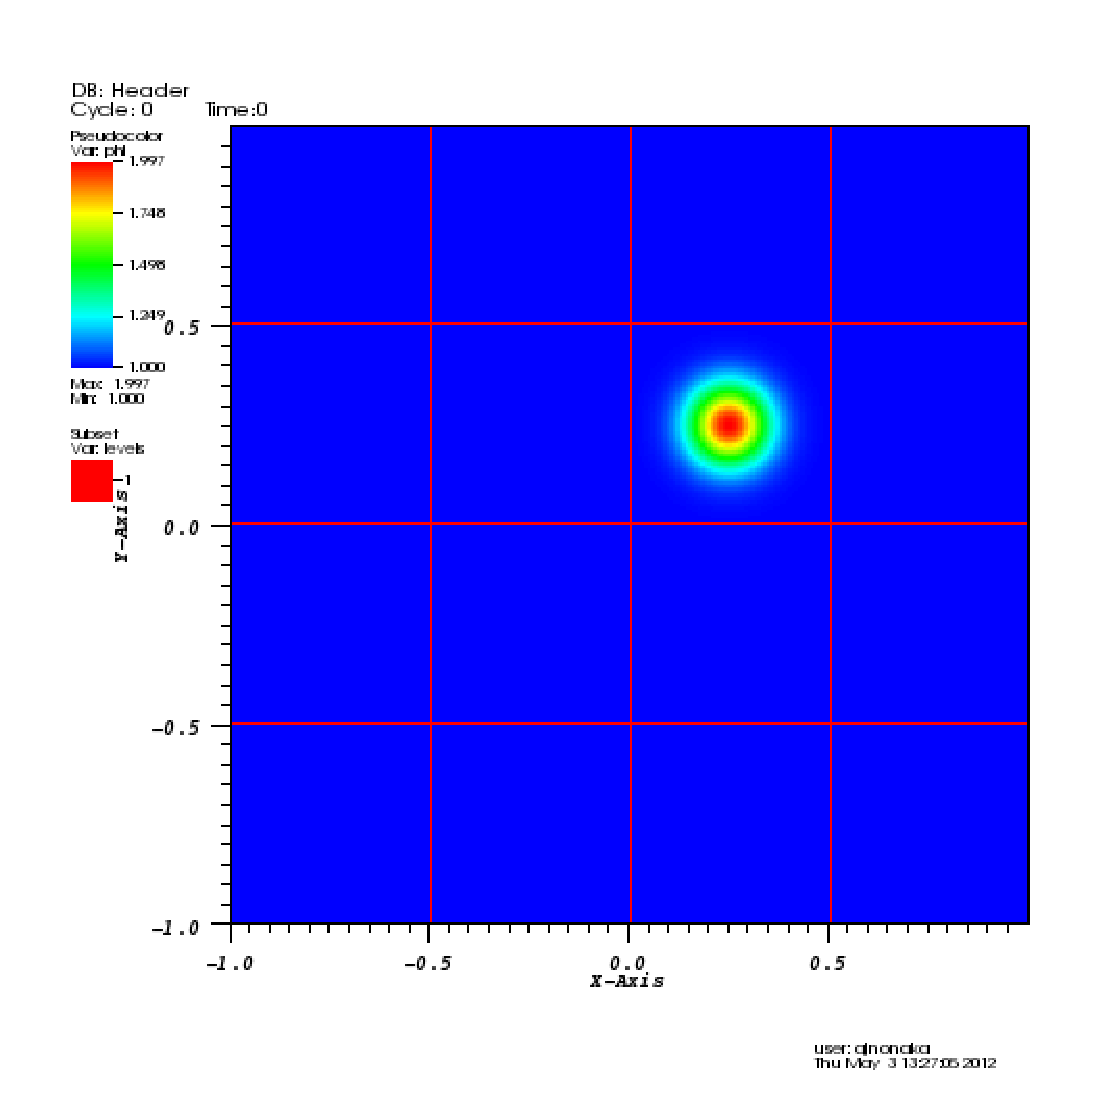
\includegraphics[width=3.1in]{./GettingStarted/VisIt_2D}
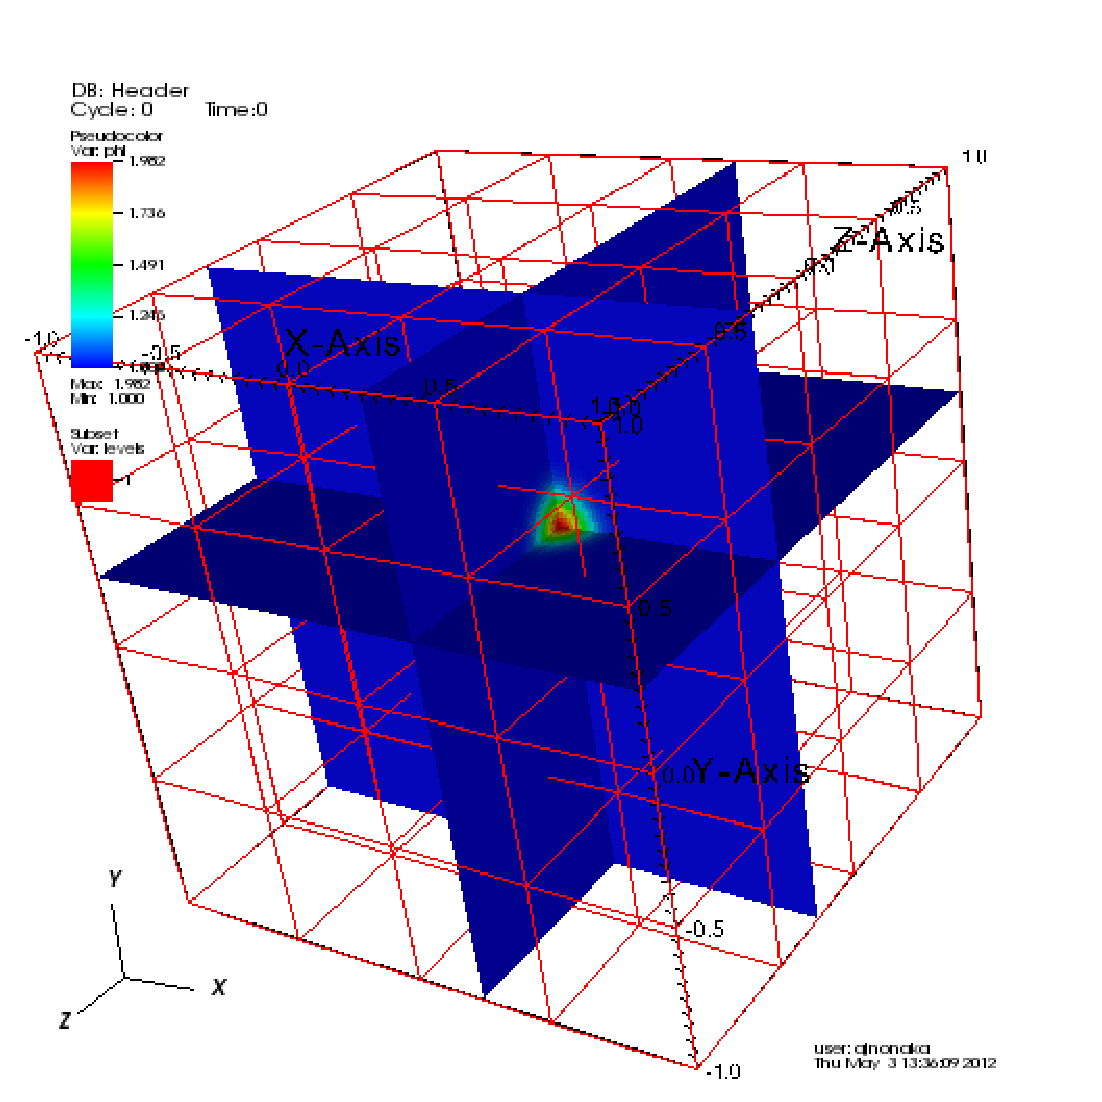
\includegraphics[width=3.1in]{./GettingStarted/VisIt_3D}
\caption{(Left) 2D image generated with VisIt.  (Right) 3D image generated with VisIt.}
\label{Fig:VisIt}
\end{figure}

In 3D, you must apply the ``Operators'' $\rightarrow$ ``Slicing'' $\rightarrow$ ``ThreeSlice'', with the 
``ThreeSlice operator attribute'' set to x=0.25, y=0.25, and z=0.25.  You can left-click and drag
over the image to rotate the image to generate something similar to right side of Figure \ref{Fig:VisIt}.\\

To make a movie, you must first create a text file named {\tt movie.visit} with a list of the {\tt Header} 
files for the individual frames.  This can most easily be done using the command:
\begin{lstlisting}[backgroundcolor=\color{light-red}].
~/BoxLib/Tutorials/HeatEquation_EX1_F> ls -1 plt*/Header | tee movie.visit
plt00000/Header
plt01000/Header
plt02000/Header
plt03000/Header
plt04000/Header
plt05000/Header
plt06000/Header
plt07000/Header
plt08000/Header
plt09000/Header
plt10000/Header
\end{lstlisting}
The next step is to run {\tt VisIt}, select ``File'' $\rightarrow$ ``Open file ...'',
then select {\tt movie.visit}.  Create an image to your liking and press the ``play'' button
on the VCR-like control panel to preview all the frames.  To save the movie, choose
``File'' $\rightarrow$ ``Save movie ...'', and follow the on-screen instructions.

\section{Running in Parallel with MPI}
We will now demonstrate how to run the example in {\tt BoxLib/Tutorials/HeatEquation\_EX1\_F/}
using MPI parallelism.  To run in parallel using C++ \BoxLib\ is analogous.
On your local machine, if you have MPI installed, you must first configure
{\tt BoxLib/Tools/F\_mk/GMakeMPI.mak} and {\tt BoxLib/Tools/C\_mk/Make.mpi}
to your MPI installation.  Then, you 
can simply build the executable as describe before, but with {\tt MPI=t} (Fortran90)
or {\tt USE\_MPI=TRUE} (C++) in the {\tt GNUmakefile}.  Alternatively, you can override the settings in 
{\tt GNUmakefile} at the command line using, e.g., ``{\tt make MPI=t}'' (Fortran90)
or ``{\tt make USE\_MPI=TRUE}'' (C++).  
An executable named {\tt main.Linux.gfortran.mpi.exe} (or similar) will be built.
Then you can run the program in parallel using, e.g.,
\begin{lstlisting}[backgroundcolor=\color{light-red}].
mpiexec -n 4 main.Linux.gfortran.mpi.ex inputs_2d
\end{lstlisting}

To run in parallel on the edison machine at NERSC, first copy the \BoxLib\ source code
into your home directory on edison and go to the {\tt HeatEquation\_EX1\_F/} directory.
The default programming environment uses the {\tt Intel} compilers.  If you want
to switch to the
{\tt gnu} programming environment to make {\tt g++} and {\tt gfortran} available,
use the command:
\begin{lstlisting}[backgroundcolor=\color{light-red}].
module swap PrgEnv-intel PrgEnv-gnu
\end{lstlisting}
Next, in {\tt GNUmakefile}, set {\tt MPI=t}, and then type ``{\tt make}''
(make sure MPI is enabled in the {\tt GNUmakefile} and the compiler is set correctly).
An executable named something like 
{\tt main2d.Linux.g++.gfortran.mpi.exe} will be built.
You cannot submit jobs in your home directory, so change to a scratch space
(``{\tt cd \$SCRATCH}'' will typically do), and copy the executable and
{\tt inputs\_2d} into this directory.  Then you need to create a job script,
e.g., "{\tt edison.run}", that has contents (for tcsh):
\lstinputlisting[backgroundcolor=\color{light-red}]{./GettingStarted/edison.run}
Note that ``-N'' and ``-n'' both indicate the number of cores you are requesting.
To run, simply type ``{\tt sbatch edison.run}''.  You can monitor the status of your job
using ``{\tt squeue -u <username>}'' and view your position in the queue 
using ``{\tt squeue}''.

\section{Running in Parallel with MPI/OpenMP (3D ONLY)}\label{Sec:OpenMP}
Both the C++ and Fortran versions of this tutorial also support hybrid MPI/OpenMP parallelism for 
{\bf three-dimensional problems only}.
You may add OMP parallelism to two-dimensional work loops, but be advised that subroutines within the \BoxLib\ infrastructure 
are not threaded for two-dimensional problems.
To ``thread'' the code, we have simply added OpenMP directives (using the {\tt !\$omp parallel do} 
construct) to any i/j/k loops we were interested in threading.  For example, in {\tt init\_phi.f90}:
\begin{lstlisting}[backgroundcolor=\color{light-green}]
!$omp parallel do private(i,j,k,x,y,z,r2)
do k=lo(3),hi(3)
   z = prob_lo(3) + (dble(k)+0.5d0) * dx
   do j=lo(2),hi(2)
      y = prob_lo(2) + (dble(j)+0.5d0) * dx
      do i=lo(1),hi(1)
         x = prob_lo(1) + (dble(i)+0.5d0) * dx

         r2 = ((x-0.25d0)**2 + (y-0.25d0)**2 + (z-0.25d0)**2) / 0.01d0
         phi(i,j,k) = 1.d0 + exp(-r2)
 
      end do
   end do
end do
!$omp end parallel do
\end{lstlisting}
This User's Guide is not a manual on OpenMP, so simply note that this particular 
construct tells each thread to work on different values of {\tt k}, with each 
thread getting its own local copy of {\tt i}, {\tt j}, {\tt x}, {\tt y}, {\tt z}, and {\tt r2}.\\

Finally, to tell the compiler that we would like to run with OpenMP, we make sure to
set {\tt OMP=t} (in Fortran) or {\tt USE\_OMP=TRUE} (in C++) in the {\tt GNUmakefile}.
Otherwise, all OpenMP directive are
simply ignored.  Note that at runtime you must have set the 
{\tt OMP\_NUM\_THREADS} environment variable properly in order for threads to work.
Also, note that you can enable/disable MPI independently from the OMP flag.  Finally,
here is a sample edison script for a hybrid MPI/OpenMP job:
\lstinputlisting[backgroundcolor=\color{light-red}]{./GettingStarted/edison_omp.run}
\begin{itemize}
\item ``-N'': number of edison nodes
\item ``-n'': total number of MPI tasks
\item ``-c'': number of threads per MPI task

\end{itemize}
